\documentclass[border=6pt]{standalone}
\usepackage[T1]{fontenc}
\usepackage{courier}
\usepackage[scaled=0.95]{helvet}
\renewcommand{\familydefault}{\sfdefault}
\usepackage{sfmath}
\usepackage[version=4]{mhchem}
\usepackage{tikz}
\usepackage{pgfplots}
\pgfplotsset{compat=newest}
\usetikzlibrary{arrows.meta,positioning,calc,fit,backgrounds,shapes.geometric,decorations.pathreplacing,patterns}
\definecolor{ink}{HTML}{17233A}
\definecolor{inksoft}{HTML}{44506A}
\definecolor{teal}{HTML}{0E6B6B}
\definecolor{tealsoft}{HTML}{E5F0EF}
\definecolor{amber}{HTML}{B26B12}
\definecolor{ambersoft}{HTML}{FBF0DF}
\definecolor{blue}{HTML}{2F6690}
\definecolor{bluesoft}{HTML}{E3ECF4}
\definecolor{plum}{HTML}{7A4D8C}
\definecolor{plumsoft}{HTML}{EFE7F3}
\definecolor{greyc}{HTML}{8A94A3}
\definecolor{linec}{HTML}{D3DCE1}
\definecolor{oxy}{HTML}{C0392B}
\definecolor{carb}{HTML}{3B4252}
\definecolor{hyd}{HTML}{E6E9EE}
\definecolor{nit}{HTML}{2F6690}
\tikzset{
  every picture/.style={line cap=round,line join=round},
  lab/.style={font=\small, text=inksoft},
  >={Stealth[length=7pt]},
}
\pgfplotsset{
  every axis/.append style={axis line style={inksoft}, tick style={inksoft}, tick label style={font=\footnotesize, text=inksoft}, label style={font=\small, text=ink}},
}
% fragment tile: \frag{node name}{position}{colour}{content}
\newcommand{\frag}[4]{\node[draw=#3, fill=#3!12, line width=1.4pt, rounded corners=6pt, minimum width=1.25cm, minimum height=1.05cm, text=#3, font=\bfseries] (#1) at (#2) {#4};}
\newcommand{\ring}{\tikz[baseline=-0.6ex]{\draw[line width=1.1pt] (0:0.3)--(60:0.3)--(120:0.3)--(180:0.3)--(240:0.3)--(300:0.3)--cycle; \draw[line width=0.8pt] (0,0) circle (0.16);}}
\newcommand{\bond}[2]{\draw[ink, line width=2.2pt] (#1) -- (#2);}

\begin{document}
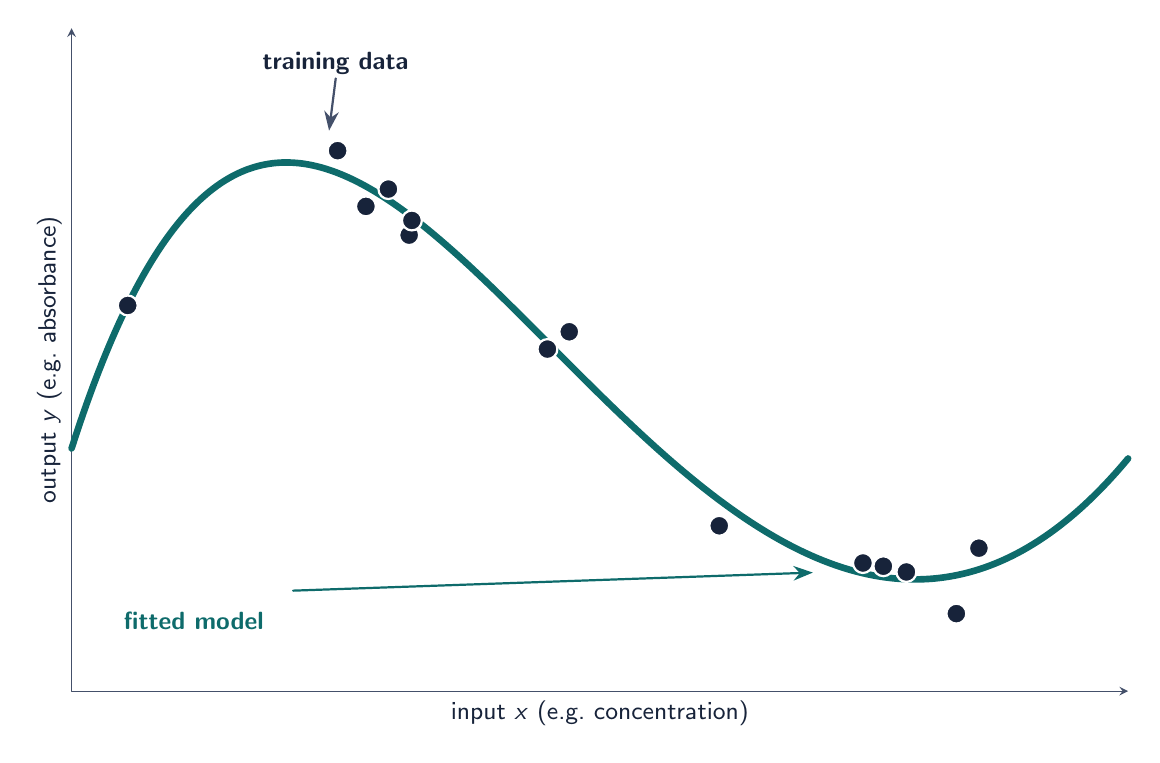
\begin{tikzpicture}
\begin{axis}[width=15cm,height=10cm,xmin=0,xmax=6.2,ymin=-1.6,ymax=1.7,
  xlabel={input $x$ (e.g.\ concentration)}, ylabel={output $y$ (e.g.\ absorbance)},
  axis lines=left, ticks=none, clip=false]
\addplot[teal, line width=2.4pt, smooth] coordinates {(0,-0.39202) (0.031156,-0.31098) (0.062312,-0.23289) (0.093467,-0.15772) (0.12462,-0.085386) (0.15578,-0.015852) (0.18693,0.050939) (0.21809,0.11504) (0.24925,0.1765) (0.2804,0.23538) (0.31156,0.29172) (0.34271,0.34557) (0.37387,0.39699) (0.40503,0.44602) (0.43618,0.49271) (0.46734,0.53711) (0.49849,0.57927) (0.52965,0.61923) (0.5608,0.65704) (0.59196,0.69274) (0.62312,0.72639) (0.65427,0.75802) (0.68543,0.78767) (0.71658,0.8154) (0.74774,0.84125) (0.77889,0.86525) (0.81005,0.88745) (0.84121,0.90789) (0.87236,0.92662) (0.90352,0.94367) (0.93467,0.95908) (0.96583,0.97289) (0.99698,0.98514) (1.0281,0.99587) (1.0593,1.0051) (1.0905,1.0129) (1.1216,1.0193) (1.1528,1.0243) (1.1839,1.028) (1.2151,1.0304) (1.2462,1.0316) (1.2774,1.0314) (1.3085,1.0301) (1.3397,1.0277) (1.3709,1.0241) (1.402,1.0194) (1.4332,1.0136) (1.4643,1.0069) (1.4955,0.99907) (1.5266,0.99031) (1.5578,0.98062) (1.5889,0.97001) (1.6201,0.95853) (1.6513,0.9462) (1.6824,0.93305) (1.7136,0.91911) (1.7447,0.9044) (1.7759,0.88896) (1.807,0.87281) (1.8382,0.85598) (1.8693,0.83849) (1.9005,0.82038) (1.9317,0.80166) (1.9628,0.78237) (1.994,0.76252) (2.0251,0.74214) (2.0563,0.72127) (2.0874,0.69991) (2.1186,0.67809) (2.1497,0.65585) (2.1809,0.63319) (2.2121,0.61015) (2.2432,0.58674) (2.2744,0.56299) (2.3055,0.53892) (2.3367,0.51454) (2.3678,0.48989) (2.399,0.46497) (2.4302,0.43982) (2.4613,0.41445) (2.4925,0.38888) (2.5236,0.36312) (2.5548,0.33721) (2.5859,0.31115) (2.6171,0.28497) (2.6482,0.25868) (2.6794,0.2323) (2.7106,0.20585) (2.7417,0.17935) (2.7729,0.15281) (2.804,0.12624) (2.8352,0.099676) (2.8663,0.073119) (2.8975,0.046588) (2.9286,0.0201) (2.9598,-0.0063309) (2.991,-0.032689) (3.0221,-0.05896) (3.0533,-0.08513) (3.0844,-0.11118) (3.1156,-0.13711) (3.1467,-0.16289) (3.1779,-0.18851) (3.209,-0.21397) (3.2402,-0.23924) (3.2714,-0.26431) (3.3025,-0.28918) (3.3337,-0.31382) (3.3648,-0.33823) (3.396,-0.3624) (3.4271,-0.38631) (3.4583,-0.40995) (3.4894,-0.43331) (3.5206,-0.45638) (3.5518,-0.47915) (3.5829,-0.50161) (3.6141,-0.52374) (3.6452,-0.54554) (3.6764,-0.567) (3.7075,-0.5881) (3.7387,-0.60884) (3.7698,-0.6292) (3.801,-0.64919) (3.8322,-0.66878) (3.8633,-0.68797) (3.8945,-0.70674) (3.9256,-0.7251) (3.9568,-0.74303) (3.9879,-0.76053) (4.0191,-0.77757) (4.0503,-0.79417) (4.0814,-0.8103) (4.1126,-0.82596) (4.1437,-0.84114) (4.1749,-0.85584) (4.206,-0.87004) (4.2372,-0.88374) (4.2683,-0.89693) (4.2995,-0.9096) (4.3307,-0.92175) (4.3618,-0.93337) (4.393,-0.94445) (4.4241,-0.95498) (4.4553,-0.96496) (4.4864,-0.97438) (4.5176,-0.98324) (4.5487,-0.99152) (4.5799,-0.99922) (4.6111,-1.0063) (4.6422,-1.0129) (4.6734,-1.0188) (4.7045,-1.0241) (4.7357,-1.0288) (4.7668,-1.0329) (4.798,-1.0363) (4.8291,-1.0391) (4.8603,-1.0413) (4.8915,-1.0429) (4.9226,-1.0437) (4.9538,-1.044) (4.9849,-1.0435) (5.0161,-1.0424) (5.0472,-1.0407) (5.0784,-1.0382) (5.1095,-1.0351) (5.1407,-1.0312) (5.1719,-1.0267) (5.203,-1.0214) (5.2342,-1.0155) (5.2653,-1.0088) (5.2965,-1.0014) (5.3276,-0.99325) (5.3588,-0.98438) (5.3899,-0.97476) (5.4211,-0.9644) (5.4523,-0.95328) (5.4834,-0.94139) (5.5146,-0.92874) (5.5457,-0.91531) (5.5769,-0.9011) (5.608,-0.8861) (5.6392,-0.8703) (5.6704,-0.85371) (5.7015,-0.8363) (5.7327,-0.81808) (5.7638,-0.79904) (5.795,-0.77916) (5.8261,-0.75845) (5.8573,-0.7369) (5.8884,-0.7145) (5.9196,-0.69124) (5.9508,-0.66711) (5.9819,-0.64211) (6.0131,-0.61623) (6.0442,-0.58946) (6.0754,-0.5618) (6.1065,-0.53323) (6.1377,-0.50375) (6.1688,-0.47334) (6.2,-0.44201)};
\addplot[only marks, mark=*, mark size=3.6pt, mark options={fill=ink, draw=white, line width=0.8pt}] coordinates {(0.32949,0.31975) (1.5612,1.0903) (1.7273,0.81304) (1.8592,0.89921) (1.9809,0.66991) (1.997,0.74291) (2.7924,0.10269) (2.9204,0.1888) (3.8005,-0.77705) (4.6438,-0.96239) (4.7636,-0.97831) (4.8989,-1.007) (5.1919,-1.2144) (5.3244,-0.88853)};
\node[font=\small\bfseries, text=ink, anchor=south] at (axis cs:1.55,1.42) {training data};
\draw[->, inksoft, thick] (axis cs:1.55,1.45) -- (axis cs:1.511,1.190);
\node[font=\small\bfseries, text=teal, anchor=west] at (axis cs:0.25,-1.25) {fitted model};
\draw[->, teal, thick] (axis cs:1.3,-1.1) -- (axis cs:4.35,-1.01);
\end{axis}
\end{tikzpicture}
\end{document}